\documentclass[12pt, openany]{book}

% NOTE: packates que se usaran en todo el proyecto
% paquetes para el idioma
\usepackage[T1]{fontenc}
\usepackage[spanish]{babel}
\defineshorthand{"-}{\babelhyphen{hard}} % para que los guiones o dashes no se fusionen

\usepackage[utf8]{inputenc}

\usepackage[top=25mm, left=25mm, bottom=25mm, right=18mm, headheight=25mm, b5paper]{geometry}

\usepackage{graphicx} % Imagenes
\usepackage{parskip} % Arreglo de la tabulación en el documento
\usepackage{xcolor, soul} % Para poder usar colores
\usepackage{titletoc} % Para personalizar la tabla de contenido
\usepackage{titlesec} % Para personalizar los títulos de los capítulos y las secciones
\usepackage{textcomp} % Agrega el paquete textcomp en el preámbulo
\usepackage{fancyhdr} % Para trabajar con el encabezado
\usepackage{amssymb} % Agrega el paquete amssymb en el preámbulo
\usepackage{listings} % Para usar el paquete listings y sintaxis de códigos
\usepackage{lipsum} % para generar texto aleatorio
\usepackage{booktabs} % Para usar tablas personalizadas.
\usepackage{lmodern} % Latin moderno
 % packages
\graphicspath{{./assets/images/}}

% Variables, colores y commandos
% Colores
\definecolor{blue_lua}{RGB}{2,2,125} % Color personalizado para el Titulo
\definecolor{base}{RGB}{48, 52, 70}
\definecolor{pink}{RGB}{195, 66, 147}
\definecolor{comment}{RGB}{165, 173, 206}
\definecolor{flamingo}{RGB}{238, 190, 190}
\definecolor{maroon}{RGB}{204, 133, 136}
\definecolor{green}{RGB}{45, 194, 89}

% Item personalizado usando el cuadrado del paquete "amssymb"
\NewDocumentCommand{\listCustom}{m}{%
	\item[\hspace{5mm}$\scriptstyle\textcolor{black!70}{\blacksquare}$\hspace{3mm}{#1}]%
}

% Para insertar codigo en linea
\newcommand{\lineCode}[1]{\colorbox{gray!10}{\textcolor{black!80}{\texttt{#1}}}}
\newcommand{\texthigh}[1]{\textcolor{black!75}{\texttt{#1}}}

\newcommand{\keyword}[1]{\textcolor{pink}{\texttt{#1}}}

% para destacar referencias
\newcommand{\textRef}[1]{\textcolor{blue!80}{\texttt{#1}}}


\renewcommand*{\familydefault}{\sfdefault} % Para que el texto sea mas bonito
\renewcommand{\headrulewidth}{0pt} % el grosor del borde del encabezado


% --------------------[config fancyhdr]-------------------------------------
\fancyhf{} % cabezera y pie de pagina vacios
% izquierdo y pares
\fancyhead[LE]{\colorbox{gray!40}{\strut{\hspace{1mm}\thepage\hspace{1mm}}}\colorbox{black!70}{\strut{\hspace{1mm}\textcolor{white}{Capítulo \thechapter}\hspace{1mm}}}}

% derecho y impares
\fancyhead[RO]{\colorbox{black!70}{\strut{\hspace{1mm}\textcolor{white}{\nouppercase{\leftmark}\hspace{1mm}}}}\colorbox{gray!40}{\strut{\hspace{1mm}\thepage\hspace{1mm}}}}

\renewcommand{\chaptermark}[1]{\markboth{#1}{}} % para filtrar "Capítulo #" y quedarse con el nombre
% ---------------------end fancyhdr ----------------------------------------

% Configuración para el lenguaje Lua
\lstdefinelanguage{Lua}{
	keywords={and, break, do, else, elseif, end, false, for, function, if, in, local, nil, not, or, repeat, return, then, true, until, while},
	sensitive=true,
	comment=[l]{--},
	string=[b]",
	string=[b]',
	morestring=[b]",
	morestring=[b]',
}

% Configuración general para mostrar código
\lstdefinestyle{mystyle}{
	backgroundcolor=\color{gray!7},
	% keywordstyle=\color{pink}, % Estilo para las palabras clave
	keywordstyle=\color{pink}\textbf,
	commentstyle=\color{comment}, % Estilo para los comentarios
	stringstyle=\color{green}, % Estilo para las cadenas de texto
	% identifierstyle=\color{white},
	identifierstyle=\color{black!80}\textit,
	basicstyle=\color{maroon},
	frame=none,
	breakatwhitespace=false,
	breaklines=true,
	keepspaces=true,
	showspaces=false,
	showstringspaces=false,
	showtabs=false,
	tabsize=3,
	% xleftmargin=10pt,                        % Margen izquierdo
	% xrightmargin=10pt,                       % Margen derecho
}

% Definir el estilo personalizado para resaltar la sintaxis de una Terminal
\lstdefinestyle{terminalstyle}{
	basicstyle=\ttfamily\color{black!80},         % Estilo de fuente y color del texto
	% backgroundcolor=\color{base},            % Color de fondo
	frame=single,                             % Borde alrededor del contenido
	xleftmargin=10pt,                        % Margen izquierdo
	xrightmargin=10pt,                       % Margen derecho
	breaklines=true,                         % Romper líneas largas
	postbreak=\mbox{\textcolor{red}{$\hookrightarrow$}\space},  % Símbolo para líneas largas rotas
	showstringspaces=false,                  % No mostrar espacios en cadenas
}


% % Personalizar el formato de los capítulos en la tabla de contenido
\titlecontents{chapter}
[0pt] % Margen izquierdo
{\vspace{10pt}\bfseries} % Formato del título de capítulo
{\contentslabel[\thecontentslabel]{10pt}} % Formato de la etiqueta de capítulo
{} % Espacio entre etiqueta y título
{\hfill\contentspage} % Formato del número de página con puntos
[\vspace{5pt}] % Espacio después de la entrada de la tabla de contenido


% Personalizar los títulos de los capítulos
\titleformat{\chapter}[display]
{\normalfont\Huge\bfseries\color{blue_lua}} % Formato del capítulo
{\bfseries\Large\itshape \thechapter} % format
{20pt} % Espacio entre la etiqueta y el título
{\Huge\color{blue_lua}} % Formato del título

% Personalizar los titulos de las secciones
\titleformat{\section}
{\normalfont\Large\bfseries} % Formato de la sección
{\color{blue!40!olive} \thesection} % Etiqueta de la sección
{10pt} % Espacio entre la etiqueta y el título
{\color{blue!40!olive}} % Formato del título


% NOTE: -------------------[Inicion]--------------------------------------------
\begin{document}


% [Página 1 - Portada]---------------------------------------------------------
\thispagestyle{empty}
\begin{center}
	
\includegraphics[width=6cm]{logo-lua-intro} % Logo de Lua

	\vspace{5mm}

	{\Huge \textcolor{blue_lua}{\textbf{Manual de Referencia de}}}

	{\Huge \textcolor{blue_lua}{\textbf{Lua 5.4}}}

	\vspace{1cm}

	Por Roberto Ierusalimschy, Luiz Henrique de Figueiredo y Waldemar Celes

\end{center}

\vfill

\begin{center}
	Copyright © 2020-2023 Lua.org, PUC-Rio. Disponible de forma gratuita bajo los términos de la licencia de Lua.
\end{center}
\newpage  % NOTE: para pasar a la siguiente pagina

% [Página 2 - pagina en blanco]------------------------------------------------
\thispagestyle{empty}
\textcolor{white}{} % truco para tener la pagina en blanco
\newpage  % NOTE: para pasar a la siguiente pagina

% [Página 3]-------------------------------------------------------------------

\thispagestyle{empty}

\textbf{Traducido y Editado por:}

Jesús Gabriel Rivera

En GitHub como \lineCode{\textit{grChad}}

\vspace{15mm}

Esta obra incluye una traducción de la documentación original de Lua, junto con contenido adicional proporcionado por mi persona. Tanto la traducción como el contenido adicional se ofrecen bajo los mismos términos y condiciones que la licencia original de Lua.

\newpage  % NOTE: para pasar a la siguiente pagina

% [Página 4 - pagina en blanco]------------------------------------------------
\thispagestyle{empty}
\textcolor{white}{} % truco para tener la pagina en blanco
\newpage  % NOTE: para pasar a la siguiente pagina

% [Página 5 - Indice General]--------------------------------------------------
\pagestyle{fancy}
\tableofcontents
\newpage  % NOTE: para pasar a la siguiente pagina

% [ Página 8 - pagina en blanco]-----------------------------------------------
\thispagestyle{empty}
\textcolor{white}{} % truco para tener la pagina en blanco
\newpage  % NOTE: para pasar a la siguiente pagina

% NOTE: Primer capitulo

\chapter{Introducción}
% \addcontentsline{toc}{chapter}{1 - Introducción}
% \setcounter{page}{1} % definir manualmente el numero de magina

Lua es un lenguaje de scripting poderoso, eficiente, liviano e integrable. Admite programación procedural, programación orientada a objetos, programación funcional, programación basada en datos y descripción de datos.

Lua combina una sintaxis procedural simple con potentes constructos de descripción de datos basados en arreglos asociativos y semánticas extensibles. Lua es de tipado dinámico, se ejecuta interpretando bytecode con una máquina virtual basada en registros y cuenta con una gestión automática de memoria con recolección de basura generacional, lo que lo hace ideal para configuración, scripting y prototipado rápido.

Lua se implementa como una biblioteca escrita en un \texthigh{C} limpio, que es un subconjunto común de \texthigh{C} estándar y \texthigh{C++}. La distribución de Lua incluye un programa principal llamado "lua", que utiliza la biblioteca Lua para ofrecer un intérprete de Lua completo e independiente, ya sea para uso interactivo o por lotes. Lua está diseñado para ser utilizado tanto como un lenguaje de scripting poderoso, liviano e integrable para cualquier programa que lo necesite, como un lenguaje independiente poderoso, liviano y eficiente.

Como lenguaje de extensión, Lua no tiene noción de un programa "principal": trabaja integrado en un cliente hospedante, llamado programa de integración o simplemente el hospedante. (Frecuentemente, este hospedante es el programa independiente "lua".) El programa hospedante puede invocar funciones para ejecutar un fragmento de código Lua, puede escribir y leer variables Lua y puede registrar funciones en C para ser llamadas por código Lua. A través del uso de funciones en C, Lua puede ser ampliado para abordar una amplia gama de dominios diferentes, creando así lenguajes de programación personalizados que comparten un marco sintáctico.

Lua es software libre y se proporciona sin garantías, como se establece en su licencia. La implementación descrita en este manual está disponible en el sitio web oficial de Lua, www.lua.org.

Al igual que cualquier otro manual de referencia, este documento puede resultar técnico en algunos lugares. Para obtener información sobre las decisiones detrás del diseño de Lua, consulte los documentos técnicos disponibles en el sitio web de Lua. Para obtener una introducción detallada a la programación en Lua, consulte el libro de Roberto, "Programming in Lua".
 % capitulo 1
% NOTE: Segundo capitulo

\chapter{Conceptos Básicos}
Esta sección describe los conceptos básicos del lenguaje.

\section{Valores y Tipos}
Lua es un lenguaje de tipado dinámico, lo que significa que las variables no tienen tipos, solo los valores los tienen. No existen definiciones de tipo en el lenguaje. Todos los valores en \texthigh{Lua} son valores de primera clase, lo que significa que se pueden almacenar en variables, pasar como argumentos a otras funciones y devolver como resultados.

Hay ocho tipos básicos en Lua: nil, boolean, number, string, function, userdata, thread y table. El tipo nil tiene un único valor, nil, cuya principal propiedad es ser diferente de cualquier otro valor; a menudo representa la ausencia de un valor útil. El tipo boolean tiene dos valores, false y true. Tanto nil como false se consideran valores falsos; se les denomina colectivamente valores falsos. Cualquier otro valor se considera verdadero. A pesar de su nombre, false se utiliza frecuentemente como una alternativa a nil, con la diferencia clave de que false se comporta como un valor regular en una tabla, mientras que un nil en una tabla representa una clave ausente.

El tipo number representa tanto números enteros como números reales (punto flotante), utilizando dos subtipos: integer (entero) y float (flotante). \texthigh{Lua} estándar utiliza enteros de 64 bits y flotantes de doble precisión (64 bits), pero también puedes compilar \texthigh{Lua} para que utilice enteros de 32 bits y/o flotantes de precisión simple (32 bits). La opción de 32 bits tanto para enteros como para flotantes es particularmente atractiva para máquinas pequeñas y sistemas integrados. (Consulta la macro LUA32BITS en el archivo luaconf.h).

A menos que se indique lo contrario, cualquier desbordamiento al manipular valores enteros realiza un ajuste, según las reglas habituales de la aritmética de complemento a dos. (En otras palabras, el resultado real es el único entero representable que es igual módulo 2n al resultado matemático, donde n es el número de bits del tipo entero).

Lua tiene reglas explícitas sobre cuándo se usa cada subtipo, pero también realiza conversiones automáticas entre ellos según sea necesario (consulte la sección 3.4.3). Por lo tanto, el programador puede optar por ignorar en su mayoría la diferencia entre enteros y flotantes, o asumir un control completo sobre la representación de cada número.

El tipo string representa secuencias inmutables de bytes. \texthigh{Lua} es compatible con 8 bits: las cadenas pueden contener cualquier valor de 8 bits, incluidos ceros incrustados ('0'). \texthigh{Lua} también es agnóstico con respecto a la codificación; no hace suposiciones sobre el contenido de una cadena. La longitud de cualquier cadena en \texthigh{Lua} debe ajustarse a un entero de Lua.

Lua puede llamar (y manipular) funciones escritas en \texthigh{Lua} y funciones escritas en \texthigh{C} (consulte la sección 3.4.10). Ambas se representan mediante el tipo function.

El tipo userdata se proporciona para permitir que los datos arbitrarios de \texthigh{C} se almacenen en variables de Lua. Un valor userdata representa un bloque de memoria sin procesar. Hay dos tipos de userdata: userdata completo, que es un objeto con un bloque de memoria administrado por Lua, y userdata ligero, que es simplemente un valor de puntero C. Los userdata no tienen operaciones predefinidas en Lua, excepto la asignación y la prueba de identidad. Mediante el uso de metatablas, el programador puede definir operaciones para valores de userdata completos (consulte la sección 2.4). Los valores userdata no se pueden crear ni modificar en Lua, solo a través de la API de C. Esto garantiza la integridad de los datos propiedad del programa hospedante y las bibliotecas de C.

El tipo thread representa hilos de ejecución independientes y se utiliza para implementar coroutines (consulte la sección 2.6). Los hilos de \texthigh{Lua} no están relacionados con los hilos del sistema operativo. \texthigh{Lua} admite coroutines en todos los sistemas, incluso aquellos que no admiten hilos nativamente.

El tipo table implementa arreglos asociativos, es decir, arreglos que pueden tener como índices no solo números, sino cualquier valor de \texthigh{Lua} excepto nil y NaN. (Not a Number es un valor especial de punto flotante utilizado por la norma IEEE 754 para representar resultados numéricos indefinidos, como 0/0). Las tablas pueden ser heterogéneas; es decir, pueden contener valores de todos los tipos (excepto nil). Cualquier clave asociada al valor nil no se considera parte de la tabla. A su vez, cualquier clave que no sea parte de una tabla tiene un valor asociado nil.

Las tablas son el único mecanismo de estructuración de datos en Lua; se pueden usar para representar arreglos ordinarios, listas, tablas de símbolos, conjuntos, registros, gráficos, árboles, etc. Para representar registros, \texthigh{Lua} utiliza el nombre del campo como índice. El lenguaje admite esta representación proporcionando a.name como azúcar sintáctica para a["name"]. Hay varias formas convenientes de crear tablas en \texthigh{Lua} (consulte la sección 3.4.9).

Al igual que los índices, los valores de los campos de la tabla pueden ser de cualquier tipo. En particular, como las funciones son valores de primera clase, los campos de la tabla pueden contener funciones. Por lo tanto, las tablas también pueden llevar métodos (consulte la sección 3.4.11).

La indexación de tablas sigue la definición de igualdad cruda en el lenguaje. Las expresiones a[i] y a[j] denotan el mismo elemento de la tabla si y solo si i y j son iguales en bruto (es decir, iguales sin metamétodos). En particular, los flotantes con valores enteros son iguales a sus respectivos enteros (por ejemplo, 1.0 == 1). Para evitar ambigüedades, cualquier flotante utilizado como clave que sea igual a un entero se convierte en ese entero. Por ejemplo, si escribes a[2.0] = true, la clave real insertada en la tabla será el entero 2.

Las tablas, funciones, hilos y valores de userdata (completos) son objetos: las variables no contienen realmente estos valores, solo referencias a ellos. La asignación, el paso de parámetros y la devolución de funciones siempre manipulan referencias a tales valores; estas operaciones no implican ningún tipo de copia.

La función de biblioteca type devuelve una cadena que describe el tipo de un valor dado (consulte type).

\section{Entornos y el Entorno Global}

Como se discutirá más adelante en las secciones 3.2 y 3.3.3, cualquier referencia a un nombre libre (es decir, un nombre no vinculado a ninguna declaración) var se traduce sintácticamente a \texthigh{\_ENV.var}. Además, cada fragmento se compila en el ámbito de una variable local externa llamada \texthigh{\_ENV} (consulte la sección 3.3.2), por lo que \texthigh{\_ENV} en sí nunca es un nombre libre en un fragmento.

A pesar de la existencia de esta variable externa \texthigh{\_ENV} y la traducción de los nombres libres,  \texthigh{\_ENV} es un nombre completamente regular. En particular, puedes definir nuevas variables y parámetros con ese nombre. Cada referencia a un nombre libre utiliza el \texthigh{\_ENV} que es visible en ese punto del programa, siguiendo las reglas habituales de visibilidad de \texthigh{Lua} (consulte la sección 3.5).

Cualquier tabla utilizada como valor de \texthigh{\_ENV} se llama entorno (environment).

Lua mantiene un entorno distinguido llamado entorno global. Este valor se guarda en un índice especial en el registro \texthigh{C} (consulte la sección 4.3). En Lua, la variable global \texthigh{\_G} se inicializa con este mismo valor. (\texthigh{\_G} no se utiliza internamente, por lo que cambiar su valor solo afectará a tu propio código).

Cuando \texthigh{Lua} carga un fragmento, el valor predeterminado para su variable \texthigh{\_ENV} es el entorno global (consulte load). Por lo tanto, de forma predeterminada, los nombres libres en el código \texthigh{Lua} se refieren a entradas en el entorno global y, por lo tanto, también se denominan variables globales. Además, todas las bibliotecas estándar se cargan en el entorno global y algunas funciones operan en ese entorno. Puedes usar load (o loadfile) para cargar un fragmento con un entorno diferente. (En \texthigh{C}, debes cargar el fragmento y luego cambiar el valor de su primer upvalue; consulta lua\_setupvalue).

\section{Manejo de Errores}

Varias operaciones en \texthigh{Lua} pueden generar un error. Un error interrumpe el flujo normal del programa, pero se puede continuar capturando el error.

El código \texthigh{Lua} puede generar explícitamente un error llamando a la función error. (Esta función nunca retorna).

Para capturar errores en Lua, puedes hacer una llamada protegida utilizando pcall (o xpcall). La función pcall llama a una función dada en modo protegido. Cualquier error que ocurra durante la ejecución de la función detiene su ejecución y el control vuelve inmediatamente a pcall, que devuelve un código de estado.

Como \texthigh{Lua} es un lenguaje de extensión incrustado, el código \texthigh{Lua} comienza a ejecutarse mediante una llamada desde el código \texthigh{C} del programa hospedante. (Cuando usas \texthigh{Lua} independiente, la aplicación lua es el programa hospedante). Por lo general, esta llamada está protegida; por lo tanto, cuando ocurre un error no protegido durante la compilación o ejecución de un fragmento Lua, el control vuelve al programa hospedante, que puede tomar medidas apropiadas, como imprimir un mensaje de error.

Cuando ocurre un error, se propaga un objeto de error con información sobre el error. \texthigh{Lua} mismo solo genera errores cuyo objeto de error es una cadena, pero los programas pueden generar errores con cualquier valor como objeto de error. Depende del programa \texthigh{Lua} o de su programa hospedante manejar dichos objetos de error. Por razones históricas, a menudo se llama mensaje de error a un objeto de error, aunque no tiene que ser una cadena.

Cuando usas xpcall (o \texthigh{lua\_pcall} en \texthigh{C}), puedes proporcionar un manejador de mensajes que se llamará en caso de errores. Esta función se llama con el objeto de error original y devuelve un nuevo objeto de error. Se llama antes de desenrollar la pila de llamadas del error, por lo que puede recopilar más información sobre el error, por ejemplo, inspeccionando la pila y creando un seguimiento de la pila (stack traceback). Este manejador de mensajes también está protegido por la llamada protegida; por lo tanto, si ocurre un error dentro del manejador de mensajes, se volverá a llamar al manejador de mensajes. Si este ciclo continúa durante demasiado tiempo, \texthigh{Lua} lo interrumpe y devuelve un mensaje apropiado. El manejador de mensajes solo se llama para errores de tiempo de ejecución regulares. No se llama para errores de asignación de memoria ni para errores durante la ejecución de finalizadores u otros manejadores de mensajes.

Lua también ofrece un sistema de advertencias (ver warn). A diferencia de los errores, las advertencias no interfieren en absoluto con la ejecución del programa. Por lo general, solo generan un mensaje al usuario, aunque este comportamiento se puede adaptar desde \texthigh{C} (ver lua\_setwarnf).

\section{Metatablas y Metamétodos}

Cada valor en \texthigh{Lua} puede tener una metatabla. Esta metatabla es una tabla \texthigh{Lua} ordinaria que define el comportamiento del valor original en ciertos eventos. Puedes cambiar varios aspectos del comportamiento de un valor estableciendo campos específicos en su metatabla. Por ejemplo, cuando un valor no numérico es el operando de una suma, \texthigh{Lua} busca una función en el campo \_\_add de la metatabla del valor. Si encuentra una, \texthigh{Lua} llama a esta función para realizar la suma.

La clave para cada evento en una metatabla es una cadena con el nombre del evento precedido por dos guiones bajos; el valor correspondiente se llama metavalue. Para la mayoría de los eventos, el metavalue debe ser una función, que luego se llama metamétodo. En el ejemplo anterior, la clave es la cadena "\_\_add" y el metamétodo es la función que realiza la suma. A menos que se indique lo contrario, un metamétodo puede ser en realidad cualquier valor invocable, que puede ser una función o un valor con un metamétodo \_\_call.

Puedes consultar la metatabla de cualquier valor utilizando la función getmetatable. \texthigh{Lua} consulta metamétodos en las metatablas utilizando un acceso directo (ver rawget).

Puedes reemplazar la metatabla de las tablas utilizando la función setmetatable. No puedes cambiar la metatabla de otros tipos desde el código Lua, excepto utilizando la biblioteca debug (sección 6.10).

Las tablas y los userdata completos tienen metatablas individuales, aunque múltiples tablas y userdata pueden compartir sus metatablas. Los valores de todos los demás tipos comparten una única metatabla por tipo; es decir, hay una única metatabla para todos los números, una para todas las cadenas, etc. Por defecto, un valor no tiene metatabla, pero la biblioteca de cadenas establece una metatabla para el tipo de cadena (ver sección 6.4).

A continuación se presenta una lista detallada de las operaciones controladas por las metatablas. Cada evento se identifica por su clave correspondiente. Por convención, todas las claves de metatablas utilizadas por \texthigh{Lua} están compuestas por dos guiones bajos seguidos de letras minúsculas del alfabeto latino.

\vspace{0.5cm}
\begin{description}
	\listCustom{\_\_add:} La operación de suma (\texthigh{+}). Si alguno de los operandos de una suma no es un número, \texthigh{Lua} intentará llamar a un metamétodo. Comienza revisando el primer operando (incluso si es un número); si ese operando no define un metamétodo para \_\_add, entonces \texthigh{Lua} revisará el segundo operando. Si \texthigh{Lua} encuentra un metamétodo, llama al metamétodo con los dos operandos como argumentos, y el resultado de la llamada (ajustado a un solo valor) es el resultado de la operación. De lo contrario, si no se encuentra ningún metamétodo, \texthigh{Lua} genera un error.

	\listCustom{\_\_sub:} La operación de resta (\texthigh{-}) tiene un comportamiento similar a la operación de suma.

	\listCustom{\_\_mul:} La operación de multiplicación (*) tiene un comportamiento similar a la operación de suma.

	\listCustom{\_\_div:} La operación de division (\texthigh{/}) tiene un comportamiento similar a la operación de suma.

	\listCustom{\_\_mod:} El operador modulo (\texthigh{\%}) tiene un comportamiento similar a la operación de suma.

	\listCustom{\_\_pow:} La operación de exponentiación (\texthigh{\textasciicircum{}}) tiene un comportamiento similar a la operación de suma.

	\listCustom{\_\_unm:} La operación de negación (unario \texthigh{-}) tiene un comportamiento similar a la operación de suma.

	\listCustom{\_\_idiv:} La operación de división entera (\texthigh{//}) tiene un comportamiento similar a la operación de suma.

	\listCustom{\_\_band:} La operación de bitwise AND (\&) tiene un comportamiento similar a la operación de suma, excepto que \texthigh{Lua} intentará utilizar un metamétodo si alguno de los operandos no es un número entero o un número de punto flotante que pueda convertirse a un entero (consulte la sección 3.4.3).

	\listCustom{\_\_bor:} La operación de bitwise OR ($\vert$) tiene un comportamiento similar a la operación de bitwise AND.

	\listCustom{\_\_bxor:} La operación de bitwise exclusive OR (\textasciitilde) tiene un comportamiento similar a la operación de bitwise AND.

	\listCustom{\_\_bnot:} La operación de bitwise NOT (\textasciitilde) tiene un comportamiento similar a la operación de bitwise AND.

	\listCustom{\_\_shl:} La operación de desplazamiento a la izquierda (\textless\textless) tiene un comportamiento similar a la operación de bitwise AND.

	\listCustom{\_\_shr:} La operación de desplazamiento a la derecha (\textgreater\textgreater) tiene un comportamiento similar a la operación de bitwise AND.

	\listCustom{\_\_concat:} La operación de concatenación (\texthigh{..}) tiene un comportamiento similar a la operación de suma. Si alguno de los operandos de la concatenación no es una cadena o un número (que siempre puede convertirse a una cadena).

	\listCustom{\_\_len:} La operación de longitud (\texthigh{\#}) tiene el siguiente comportamiento: si el objeto no es una cadena, \texthigh{Lua} intentará utilizar su metamétodo. Si existe un metamétodo, \texthigh{Lua} lo llama con el objeto como argumento y el resultado de la llamada (siempre ajustado a un solo valor) es el resultado de la operación. Si no hay metamétodo pero el objeto es una tabla, entonces \texthigh{Lua} utiliza la operación de longitud de la tabla (ver sección 3.4.7). De lo contrario, \texthigh{Lua} genera un error.

	\listCustom{\_\_eq:} La operación de igualdad (\texthigh{==}) tiene un comportamiento similar a la operación de suma. Sin embargo, \texthigh{Lua} intentará utilizar un metamétodo solo cuando los valores que se están comparando sean ambas tablas o ambos userdata completos, y no sean primitivamente iguales. El resultado de la llamada siempre se convierte en un valor booleano.

	\listCustom{\_\_lt:} La operación de menor que (\textless) tiene un comportamiento similar a la operación de suma. Sin embargo, \texthigh{Lua} intentará utilizar un metamétodo solo cuando los valores que se están comparando no sean ambos números ni ambas cadenas. Además, el resultado de la llamada siempre se convierte en un valor booleano.

	\listCustom{\_\_le:} La operación de menor o igual que (\textless=) tiene un comportamiento similar a la operación de menor que (\textless).

	\listCustom{\_\_index:} La operación de acceso de índice \lineCode{table[key]} ocurre cuando \texthigh{table} no es una tabla o cuando \texthigh{key} no está presente en \texthigh{table}. El metavalue se busca en la metatabla de \texthigh{table}.

	El metavalue para este evento puede ser una función, una tabla o cualquier valor con un metavalue \texthigh{\_\_index}. Si es una función, se llama con \texthigh{table} y \texthigh{key} como argumentos, y el resultado de la llamada (ajustado a un solo valor) es el resultado de la operación. De lo contrario, el resultado final es el resultado de indexar este metavalue con \texthigh{key}. Esta indexación es regular, no raw, por lo tanto puede activar otro metavalue \texthigh{\_\_index}.

	\listCustom{\_\_newindex:} La asignación de índice \lineCode{table[key] = value} ocurre cuando \texthigh{table} no es una tabla o cuando \texthigh{key} no está presente en \texthigh{table}. El metavalue se busca en la metatabla de \texthigh{table}.

	Al igual que con la indexación, el metavalue para este evento puede ser una función, una tabla o cualquier valor con un metavalue \texthigh{\_\_newindex}. Si es una función, se llama con \texthigh{table}, \texthigh{key} y \texthigh{value} como argumentos. De lo contrario, \texthigh{Lua} repite la asignación de índice sobre este metavalue con la misma key y value. Esta asignación es regular, no raw, por lo tanto puede activar otro metavalue \texthigh{\_\_newindex}.

	Cuando se invoca un metavalue \texthigh{\_\_newindex}, \texthigh{Lua} no realiza la asignación primitiva. Si es necesario, el metamétodo en sí puede llamar a \textcolor{blue!80}{\texthigh{rawset}} para realizar la asignación.

	\listCustom{\_\_call:} La operación de llamada \lineCode{func(args)} ocurre cuando \texthigh{Lua} intenta llamar a un valor que no es una función (es decir, \texthigh{func} no es una función). Se busca el metamétodo en \texthigh{func}. Si está presente, se llama al metamétodo con \texthigh{func} como primer argumento, seguido de los argumentos de la llamada original (\texthigh{args}). Todos los resultados de la llamada son los resultados de la operación. Este es el único metamétodo que permite múltiples resultados.

\end{description}

\vspace{0.5cm} % espacio de 0.5 centimetros

Además de la lista anterior, el intérprete también respeta las siguientes claves en las metatablas: \texthigh{\_\_gc} (ver sección 2.5.3), \texthigh{\_\_close} (ver sección 3.3.8), \texthigh{\_\_mode} (ver sección 2.5.4) y \texthigh{\_\_name}. (La entrada \texthigh{\_\_name}, cuando contiene una cadena, puede ser utilizada por \textRef{tostring} y en mensajes de error).

Para los operadores unarios (negación, longitud y bitwise NOT), el metamétodo se calcula y se llama con un segundo operando ficticio igual al primero. Este operando adicional solo se utiliza para simplificar los aspectos internos de \texthigh{Lua} (haciendo que estos operadores se comporten como una operación binaria) y puede ser eliminado en futuras versiones. Para la mayoría de los casos de uso, este operando adicional no es relevante.

Dado que las metatablas son tablas regulares, pueden contener campos arbitrarios, no solo los nombres de eventos mencionados anteriormente. Algunas funciones de la biblioteca estándar (por ejemplo, \textRef{tostring}) utilizan otros campos en las metatablas para sus propios propósitos.

Es una buena práctica agregar todos los metamétodos necesarios a una tabla antes de establecerla como metatabla de algún objeto. En particular, el metamétodo \texthigh{\_\_gc} funciona solo cuando se sigue este orden (ver sección 2.5.3). También es una buena práctica establecer la metatabla de un objeto justo después de su creación.

\section{Recolección de Basura}

Lua realiza la gestión automática de memoria. Esto significa que no tienes que preocuparte por asignar memoria para nuevos objetos ni liberarla cuando los objetos ya no sean necesarios. \texthigh{Lua} administra la memoria automáticamente ejecutando un \emph{recolector de basura o (Garbage Collector)} para recoger todos los objetos muertos. Toda la memoria utilizada por \texthigh{Lua} está sujeta a una gestión automática: cadenas, tablas, userdata, funciones, hilos, estructuras internas, etc.

Un objeto se considera muerto en cuanto el recolector puede estar seguro de que el objeto no será accedido nuevamente en la ejecución normal del programa. ("Ejecución normal" aquí excluye los finalizadores, que pueden resucitar objetos muertos (ver sección 2.5.3), y también excluye las operaciones que utilizan la biblioteca de depuración). Es importante tener en cuenta que el momento en que el recolector puede estar seguro de que un objeto está muerto puede no coincidir con las expectativas del programador. La única garantía es que \texthigh{Lua} no recogerá un objeto que aún pueda ser accedido en la ejecución normal del programa, y eventualmente recogerá un objeto que sea inaccesible desde Lua. (Aquí, \emph{inaccesible desde Lua} significa que ni una variable ni otro objeto vivo hacen referencia al objeto). Debido a que \texthigh{Lua} no tiene conocimiento sobre el código \texthigh{C}, nunca recoge objetos accesibles a través del registro (ver sección 4.3), que incluye el entorno global (ver sección 2.2).

El recolector de basura (GC o Garbage Collector) en \texthigh{Lua} puede trabajar en dos modos: incremental y generacional.

El modo GC predeterminado con los parámetros predeterminados es adecuado para la mayoría de los casos de uso. Sin embargo, los programas que desperdician una gran proporción de su tiempo asignando y liberando memoria pueden beneficiarse de otros ajustes. Ten en cuenta que el comportamiento del GC no es portátil tanto entre plataformas como entre diferentes versiones de Lua; por lo tanto, los ajustes óptimos tampoco son portátiles.

Puedes cambiar el modo y los parámetros del GC llamando a \textRef{lua\_gc} en \texthigh{C} o \textRef{collectgarbage} en Lua. También puedes usar estas funciones para controlar el recolector directamente (por ejemplo, para detenerlo y reiniciarlo).

\subsection{Recolección de Basura Incremental}

En el modo incremental, cada ciclo del recolector de basura realiza una colección de marcas y barrido en pequeños pasos entrelazados con la ejecución del programa. En este modo, el recolector utiliza tres números para controlar sus ciclos de recolección de basura: el \textit{garbage-collector pause}, el \textit{garbage-collector step multiplier} y el \textit{garbage-collector step size}.

El \lineCode{garbage-collector pause} controla cuánto tiempo espera el recolector antes de comenzar un nuevo ciclo. El recolector inicia un nuevo ciclo cuando el uso de memoria alcanza \texthigh{\emph{n\%}} del uso después de la recolección anterior. Valores más grandes hacen que el recolector sea menos agresivo. Los valores iguales o inferiores a 100 significan que el recolector no esperará para comenzar un nuevo ciclo. Un valor de 200 significa que el recolector espera que el uso total de memoria se duplique antes de comenzar un nuevo ciclo. El valor predeterminado es 200; el valor máximo es 1000.

El \lineCode{garbage-collector step multiplier} controla la velocidad del recolector en relación con la asignación de memoria, es decir, cuántos elementos marca o barre por cada kilobyte de memoria asignada. Valores más grandes hacen que el recolector sea más agresivo, pero también aumentan el tamaño de cada paso incremental. No se deben usar valores inferiores a 100, porque hacen que el recolector sea demasiado lento y pueden hacer que el recolector nunca termine un ciclo. El valor predeterminado es 100; el valor máximo es 1000.

El \lineCode{garbage-collector step sizes} controla el tamaño de cada paso incremental, específicamente cuántos bytes asigna el intérprete antes de realizar un paso. Este parámetro es logarítmico: un valor de \texthigh{\textit{n}} significa que el intérprete asignará $2^n$ bytes entre pasos y realizará un trabajo equivalente durante el paso. Un valor grande (por ejemplo, 60) hace que el recolector sea un recolector de detención del mundo (no incremental). El valor predeterminado es 13, lo que significa pasos de aproximadamente 8 Kbytes.

\subsection{Recolección de Basura Generacional}

En el modo generacional, el recolector realiza colecciones menores frecuentes, que recorren solo los objetos creados recientemente. Si después de una colección menor el uso de memoria sigue por encima de un límite, el recolector realiza una colección mayor de detención del mundo, que recorre todos los objetos. El modo generacional utiliza dos parámetros: el \textit{minor multiplier} y el \textit{major multiplier}.

El \lineCode{minor multiplier} controla la frecuencia de las colecciones menores. Para un multiplicador menor \texthigh{\emph{x}}, se realizará una nueva colección menor cuando la memoria crezca \texthigh{\emph{x\%}} más grande que la memoria en uso después de la colección mayor anterior. Por ejemplo, para un multiplicador de 20, el recolector realizará una colección menor cuando el uso de memoria sea un 20\% más grande que el uso después de la colección mayor anterior. El valor predeterminado es 20; el valor máximo es 200.

El \lineCode{major multiplier} controla la frecuencia de las colecciones mayores. Para un multiplicador mayor \texthigh{\emph{x}}, se realizará una nueva colección mayor cuando la memoria crezca \texthigh{\emph{x\%}} más grande que la memoria en uso después de la colección mayor anterior. Por ejemplo, para un multiplicador de 100, el recolector realizará una colección mayor cuando el uso de memoria sea más grande que el doble del uso después de la colección anterior. El valor predeterminado es 100; el valor máximo es 1000.

\subsection{Metamétodos de Recolección de Basura}

Puedes establecer metamétodos del recolector de basura (finalizadores) para tablas y, utilizando la API de \texthigh{C}, para full userdata (ver sección 2.4). Estos finalizadores son llamados cuando el recolector de basura de \texthigh{Lua} detecta que la tabla o userdata correspondiente está marcada como inaccesible. Los finalizadores te permiten coordinar la recolección de basura de \texthigh{Lua} con la gestión externa de recursos, como cerrar archivos, conexiones de red o bases de datos, o liberar tu propia memoria.

Para que un objeto (tabla o userdata) sea finalizado cuando se recolecta, debes marcarlo para finalización. Marcas un objeto para finalización cuando le asignas su metatabla y la metatabla tiene un metamétodo \texthigh{\_\_gc}. Ten en cuenta que si estableces una metatabla sin un campo \texthigh{\_\_gc} y más tarde creas ese campo en la metatabla, el objeto no se marcará para finalización.

Cuando un objeto marcado se vuelve inaccesible, no es recolectado inmediatamente por el recolector de basura de \texttt{Lua}. En su lugar, \texthigh{Lua} lo pone en una lista. Después de la recolección, \texthigh{Lua} recorre esa lista. Para cada objeto en la lista, verifica el metamétodo \texthigh{\_\_gc} del objeto: Si está presente, \texthigh{Lua} lo llama con el objeto como su único argumento.

Al final de cada ciclo de recolección de basura, los finalizadores son llamados en orden inverso a cómo los objetos fueron marcados para finalización, entre los objetos recolectados en ese ciclo; es decir, el primer finalizador en ser llamado es aquel asociado al objeto marcado en último lugar en el programa. La ejecución de cada finalizador puede ocurrir en cualquier momento durante la ejecución del código regular.

Dado que el objeto que está siendo recolectado todavía debe ser utilizado por el finalizador, ese objeto (y otros objetos accesibles solo a través de él) deben ser resucitados por \texthigh{Lua}. Por lo general, esta resurrección es transitoria, y la memoria del objeto se libera en el siguiente ciclo de recolección de basura. Sin embargo, si el finalizador almacena el objeto en algún lugar global (por ejemplo, una variable global), entonces la resurrección es permanente. Además, si el finalizador marca un objeto en proceso de finalización para finalización nuevamente, su finalizador será llamado nuevamente en el siguiente ciclo donde el objeto esté inaccesible. En cualquier caso, la memoria del objeto se libera solo en un ciclo de recolección de basura donde el objeto esté inaccesible y no marcado para finalización.

Cuando cierras un estado de \texthigh{Lua} (ver \textRef{lua\_close}), \texthigh{Lua} llama a los finalizadores de todos los objetos marcados para finalización, siguiendo el orden inverso en que fueron marcados. Si algún finalizador marca objetos para recolección durante esa fase, esas marcas no tienen efecto.

Los finalizadores no pueden pausar ni ejecutar el recolector de basura. Debido a que pueden ejecutarse en momentos impredecibles, es una buena práctica restringir cada finalizador al mínimo necesario para liberar adecuadamente su recurso asociado.

Cualquier error mientras se ejecuta un finalizador genera una advertencia; el error no se propaga.

\subsection{Tablas Débiles}

Una tabla débil (weak table) es una tabla cuyos elementos son referencias débiles. Una referencia débil es ignorada por el recolector de basura. En otras palabras, si las únicas referencias a un objeto son referencias débiles, entonces el recolector de basura recolectará ese objeto.

Una tabla débil puede tener claves débiles, valores débiles, o ambas. Una tabla con valores débiles permite la recolección de sus valores, pero evita la recolección de sus claves. Una tabla con claves débiles y valores débiles permite la recolección tanto de claves como de valores. En cualquier caso, si tanto la clave como el valor son recolectados, el par completo se elimina de la tabla. La debilidad de una tabla está controlada por el campo \texthigh{\_\_mode} de su metatabla. Este metavalue, si está presente, debe ser una de las siguientes cadenas: \textit{"k"}, para una tabla con claves débiles; \textit{"v"}, para una tabla con valores débiles; o \textit{"kv"}, para una tabla con ambas claves y valores débiles.

Una tabla con claves débiles y valores fuertes también se llama tabla efímera (ephemeron). En una tabla efímera, se considera que un valor es alcanzable solo si su clave es alcanzable. En particular, si la única referencia a una clave proviene de su valor, el par se elimina.

Cualquier cambio en la debilidad de una tabla puede surtir efecto solo en el próximo ciclo de recolección. En particular, si cambias la debilidad a un modo más fuerte, \texthigh{Lua} puede seguir recolectando algunos elementos de esa tabla antes de que el cambio surta efecto.

Solo los objetos que tienen una construcción explícita se eliminan de las tablas débiles. Los valores, como los números y las funciones \texthigh{C} ligeras, no están sujetos a la recolección de basura y, por lo tanto, no se eliminan de las tablas débiles (a menos que se recolecten sus valores asociados). Aunque las cadenas están sujetas a la recolección de basura, no tienen una construcción explícita y su igualdad es por valor; se comportan más como valores que como objetos. Por lo tanto, no se eliminan de las tablas débiles.

Los objetos resucitados (es decir, objetos en proceso de finalización y objetos accesibles solo a través de objetos en proceso de finalización) tienen un comportamiento especial en las tablas débiles. Se eliminan de los valores débiles antes de ejecutar sus finalizadores, pero solo se eliminan de las claves débiles en la próxima recolección después de ejecutar sus finalizadores, cuando estos objetos son liberados efectivamente. Este comportamiento permite que el finalizador acceda a propiedades asociadas con el objeto a través de tablas débiles.

Si una tabla débil se encuentra entre los objetos resucitados en un ciclo de recolección, es posible que no se limpie correctamente hasta el siguiente ciclo.

\section{Coroutines}

\texthigh{Lua} admite coroutines, también llamadas \textit{collaborative multithreading}. Una coroutine en \texthigh{Lua}  representa un hilo de ejecución independiente. Sin embargo, a diferencia de los hilos en sistemas de multiprocesamiento, una coroutine solo suspende su ejecución mediante una llamada explícita a la función yield.

Se crea una coroutine llamando a \textRef{coroutine.create}. Su único argumento es una función que es la función principal de la coroutine. La función create solo crea una nueva coroutine y devuelve un identificador para ella (un objeto de \textit{type thread}); no inicia la coroutine.

Se ejecuta una coroutine llamando a \textRef{coroutine.resume}. Cuando se llama por primera vez a \textRef{coroutine.resume}, pasando como primer argumento un hilo devuelto por \textRef{coroutine.create}, la coroutine comienza su ejecución llamando a su función principal. Los argumentos adicionales pasados a \textRef{coroutine.resume} se pasan como argumentos a esa función. Después de que la coroutine comienza a ejecutarse, se ejecuta hasta que termina o hace un \textit{yield}.

Una coroutine puede terminar su ejecución de dos maneras: de manera normal, cuando su función principal retorna (explícitamente o implícitamente, después de la última instrucción); y de manera anormal, si hay un error no protegido. En caso de terminación normal, \textRef{coroutine.resume} devuelve \textbf{true}, más cualquier valor devuelto por la función principal de la coroutine. En caso de errores, \textRef{coroutine.resume} devuelve \textbf{false} más el objeto de error. En este caso, la coroutine no desenrolla su pila, por lo que es posible inspeccionarla después del error con la API de depuración.

Una coroutine hace un yield llamando a \textRef{coroutine.yield}. Cuando una coroutine hace un yield, la llamada correspondiente a \textRef{coroutine.resume} devuelve inmediatamente, incluso si el yield ocurre dentro de llamadas de función anidadas (es decir, no en la función principal, sino en una función llamada directa o indirectamente por la función principal). En el caso de un yield, \textRef{coroutine.resume} también devuelve \textbf{true}, más cualquier valor pasado a \textRef{coroutine.yield}. La próxima vez que se reanuda la misma coroutine, continúa su ejecución desde el punto donde hizo el yield, y la llamada a \textRef{coroutine.yield} devuelve cualquier argumento adicional pasado a \textRef{coroutine.resume}.

Al igual que \textRef{coroutine.create}, la función \textRef{coroutine.wrap} también crea una coroutine, pero en lugar de devolver la coroutine en sí misma, devuelve una función que, cuando se llama, reanuda la coroutine. Cualquier argumento pasado a esta función se pasa como argumentos adicionales a \textRef{coroutine.resume}. \textRef{coroutine.wrap} devuelve todos los valores devueltos por \textRef{coroutine.resume}, excepto el primero (el código de error booleano). A diferencia de \textRef{coroutine.resume}, la función creada por \textRef{coroutine.wrap} propaga cualquier error al llamador. En este caso, la función también cierra la coroutine (ver \textRef{coroutine.close}).

\vspace{5mm} % Espacio vertical de 5mm
Como ejemplo de cómo funcionan las coroutines, considera el siguiente código:

\begin{lstlisting}[language=Lua, style=mystyle]
  function foo()
    print("foo", a)
    return coroutine.yield(2 * a)
  end

  co = coroutine.create(function(a, b)
    print("co-boby", a, b)
    local r = foo(a + 1)
    print("co-boby", r)
    local r, s = coroutine.yield(a + b, a - b)
    print("co-boby", r, s)
    return b, "end"
  end)

  print("main", coroutine.resume(co, 1, 10))
  print("main", coroutine.resume(co, "r"))
  print("main", coroutine.resume(co, "x", "y"))
  print("main", coroutine.resume(co, "x", "y"))
\end{lstlisting}

\newpage

Cuando lo ejecutas, produce la siguiente salida:

\begin{center}
	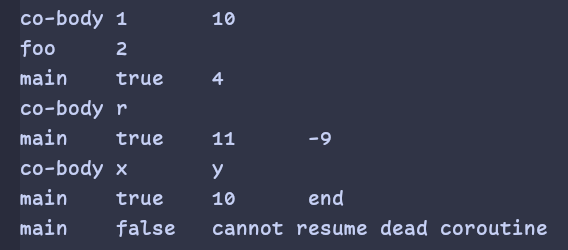
\includegraphics[width=9cm]{chapter2/console01} % imagen de la salida de consola
\end{center}

\vspace{5mm} % Espacio vertical de 5mm

También puedes crear y manipular coroutines a través de la API de C: consulta las funciones \textRef{lua\_newthread}, \textRef{lua\_resume} y \textRef{lua\_yield}.
 % capitulo 2
% NOTE: Chapter 03

\chapter{El Lenguaje}
Esta sección describe el léxico, la sintaxis y la semántica de \texthigh{Lua}. En otras palabras, esta sección describe qué tokens son válidos, cómo pueden combinarse y qué significan sus combinaciones.

Los constructos del lenguaje se explicarán utilizando la notación BNF extendida habitual, en la que \lineCode{\{a\}} significa \texthigh{0} o más \texthigh{a's}, y \lineCode{[a]} significa un \texthigh{a} opcional. Los no terminales se muestran como non-terminal, las palabras clave se muestran como \textbf{kword} y otros símbolos terminales se muestran como '='. La sintaxis completa de \texthigh{Lua} se puede encontrar en la sección 9 al final de este manual.


% NOTE: [Primera sección]------------------------------------------------------
\section{Convenciones léxicas}
\texthigh{Lua} es un lenguaje de formato libre. Ignora los espacios y los comentarios entre elementos léxicos (tokens), excepto como delimitadores entre dos tokens. En el código fuente, \texthigh{Lua} reconoce como espacios los caracteres de espacio en blanco ASCII estándar: espacio, avance de formulario, nueva línea, retorno de carro, tabulación horizontal y tabulación vertical.

Los nombres (también llamados identificadores) en \texthigh{Lua} pueden ser cualquier cadena de letras latinas, dígitos arábigos y guiones bajos, que no comience con un dígito y no sea una palabra reservada. Los identificadores se utilizan para nombrar variables, campos de tablas y etiquetas.

Las siguientes palabras clave están reservadas y no pueden ser utilizadas como nombres:

\begin{center} % Centrar la tabla en el texto
	\begin{tabular}{llllll} % Definición de las columnas y el formato de la tabla
		% \toprule % Línea horizontal superior
		\keyword{and}   & \keyword{break} & \keyword{do}       & \keyword{else}  & \keyword{elseif} & \keyword{end}    \\ % Contenido de la primera fila
		\keyword{false} & \keyword{for}   & \keyword{function} & \keyword{goto}  & \keyword{if}     & \keyword{in}     \\ % Contenido de la segunda fila
		\keyword{local} & \keyword{nil}   & \keyword{not}      & \keyword{or}    & \keyword{repeat} & \keyword{return} \\ % Contenido de la tercera fila
		\keyword{then}  & \keyword{true}  & \keyword{until}    & \keyword{while}                                       \\ % Contenido de la cuarta fila \bottomrule % Línea horizontal inferior
	\end{tabular}
	\label{tab:keywords} % Etiqueta para referenciar la tabla
\end{center}

\texthigh{Lua} es un lenguaje sensible a mayúsculas y minúsculas: \keyword{and} es una palabra reservada, pero 'And' y 'AND' son dos nombres diferentes y válidos. Como convención, los programas deben evitar crear nombres que comiencen con un guión bajo seguido de una o más letras mayúsculas (como \_VERSION).

Las siguientes cadenas de texto representan otros tokens:
\begin{center}
	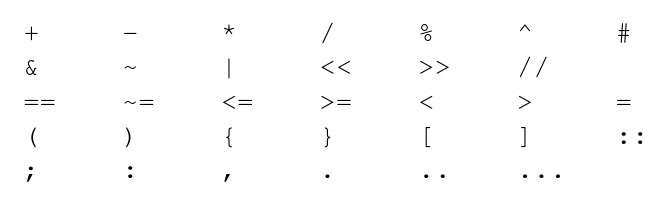
\includegraphics[width=10cm]{chapter3/strings-tokens} % imagen de los tokens
\end{center}

Una cadena de texto corta (literal) puede estar delimitada por comillas simples o comillas dobles y puede contener las siguientes secuencias de escape similares a las de C: '\texthigh{\textbackslash{a}}' (campana), '\texthigh{\textbackslash{b}}' (backspace), '\texthigh{\textbackslash{f}}' (avance de página), '\texthigh{\textbackslash{n}}' (nueva línea), '\texthigh{\textbackslash{r}}' (retorno de carro), '\texthigh{\textbackslash{t}}' (tabulación horizontal), '\texthigh{\textbackslash{v}}' (tabulación vertical), '\texthigh{\textbackslash \textbackslash}' (backslash), '\texthigh{\textbackslash "}' (comilla doble) y '\texthigh{\textbackslash '}' (comilla simple). Si un carácter barra invertida se sigue de un salto de línea, esto resulta en una nueva línea en la cadena de texto. La secuencia de escape '\texthigh{\textbackslash{z}}' omite el siguiente conjunto de caracteres de espacio en blanco, incluyendo saltos de línea; esto es especialmente útil para dividir e indentar una cadena de texto larga en varias líneas sin agregar los saltos de línea y espacios en el contenido de la cadena. Una cadena de texto corta no puede contener saltos de línea no escapados ni secuencias de escape que no formen una secuencia de escape válida.

En una cadena de texto corta (literal), podemos especificar cualquier byte, incluso ceros incrustados, mediante su valor numérico. Esto se puede hacer utilizando la secuencia de escape \texthigh{\textbackslash{xXX}}, donde \texthigh{XX} es una secuencia de exactamente dos dígitos hexadecimales, o con la secuencia de escape \texthigh{\textbackslash{ddd}}, donde \texthigh{ddd} es una secuencia de hasta tres dígitos decimales. (Tenga en cuenta que si una secuencia de escape decimal debe ir seguida de un dígito, debe expresarse con exactamente tres dígitos).

La codificación UTF-8 de un carácter Unicode se puede insertar en una cadena de texto corta (literal) con la secuencia de escape \texthigh{\textbackslash{u\{XXX\}}} (con las llaves obligatorias), donde \texthigh{XXX} es una secuencia de uno o más dígitos hexadecimales que representan el punto de código del carácter. Este punto de código puede tener cualquier valor menor que $2^{31}$. (\texthigh{Lua} utiliza la especificación original de UTF-8 aquí, que no está restringida a puntos de código Unicode válidos).

Las cadenas de texto literales también se pueden definir utilizando un formato largo, que está encerrado por corchetes largos. Definimos un corchete largo de apertura de nivel n como un corchete cuadrado de apertura seguido de n signos de igual seguidos por otro corchete cuadrado de apertura. Así, un corchete largo de apertura de nivel 0 se escribe como \texthigh{[[}, un corchete largo de apertura de nivel 1 se escribe como \texthigh{[=[}, y así sucesivamente. Un corchete largo de cierre se define de manera similar; por ejemplo, un corchete largo de cierre de nivel 4 se escribe como \texthigh{]====]}. Una cadena larga comienza con un corchete largo de apertura de cualquier nivel y termina en el primer corchete largo de cierre del mismo nivel. Puede contener cualquier texto excepto un corchete de cierre del mismo nivel. Las cadenas literales en esta forma entre corchetes pueden extenderse por varias líneas, no interpretan secuencias de escape y ignoran corchetes largos de cualquier otro nivel. Cualquier tipo de secuencia de fin de línea (retorno de carro, nueva línea, retorno de carro seguido de nueva línea o nueva línea seguida de retorno de carro) se convierte en una simple nueva línea. Cuando el corchete largo de apertura está inmediatamente seguido de una nueva línea, la nueva línea no se incluye en la cadena.

Como ejemplo, en un sistema que utiliza ASCII (en el cual '\texthigh{a}' está codificado como 97, newline está codificada como 10 y '\texthigh{1}' está codificado como 49), las cinco cadenas literales siguientes denotan la misma cadena:

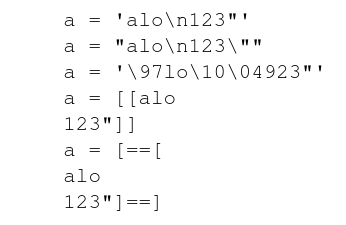
\includegraphics[width=6cm]{chapter3/example01} % imagen de ejemplo

Cualquier byte en una cadena literal que no esté explícitamente afectado por las reglas anteriores se representa tal cual. Sin embargo, \texthigh{Lua} abre archivos para su análisis en modo de texto y las funciones del sistema para archivos pueden tener problemas con algunos caracteres de control. Por lo tanto, es más seguro representar datos binarios como una cadena literal con secuencias de escape explícitas para los caracteres que no son de texto.

Una constante numérica (o numeral) en \texthigh{Lua} puede escribirse con una parte fraccional opcional y un exponente decimal opcional, marcado con una letra '\texthigh{e}' o '\texthigh{E}'. \texthigh{Lua} también acepta constantes hexadecimales, que comienzan con \texthigh{0x} o \texthigh{0X}. Las constantes hexadecimales también pueden tener una parte fraccional opcional y un exponente binario opcional, marcado con una letra '\texthigh{p}' o '\texthigh{P}' y escrito en decimal. (Por ejemplo, \texthigh{0x1}.\texthigh{fp10} representa el número 1984, que es 0x1f dividido con 16 y  multiplicado por $2^{10}$ ---> \lineCode{(0x1f/16)*$2^{10}$}).

Una constante numérica con un punto decimal o un exponente denota un número de tipo "float" (número de punto flotante); de lo contrario, si su valor cabe en un número entero o es una constante hexadecimal, denota un número entero; de lo contrario (es decir, si es un número entero decimal que desborda), denota un número de tipo "float". Los números hexadecimales sin punto decimal ni exponente siempre denotan un valor entero; si el valor desborda, se ajusta para que entre en un entero válido.

Ejemplos de constantes enteras válidas son:

\begin{center}
	\begin{tabular}{llll} % Definición de las columnas y el formato de la tabla
		\texthigh{3} & \texthigh{345} & \texthigh{0xff} & \texthigh{0xBEBADA} \\
	\end{tabular}
	\label{tab:ejemplo} % Etiqueta para referenciar la tabla
\end{center}

Ejemplos de constantes flotantes válidas son:

\begin{center}
	\begin{tabular}{lllll} % Definición de las columnas y el formato de la tabla
		\texthigh{3.0}    & \texthigh{3.1416}   & \texthigh{314.16e-2}            & \texthigh{0.31416E1} & \texthigh{34e1} \\
		\texthigh{0x0.1E} & \texthigh{0xA23p-4} & \texthigh{0X1.921FB54442D18P+1}                                          \\
	\end{tabular}
	\label{tab:ejemplo} % Etiqueta para referenciar la tabla
\end{center}

Un comentario comienza con dos guiones medios ("--) en cualquier lugar fuera de una cadena. Si el texto inmediatamente después de "-- no es un corchete largo de apertura, el comentario es un comentario corto, que se extiende hasta el final de la línea. De lo contrario, es un comentario largo, que se extiende hasta el corchete largo de cierre correspondiente.


% NOTE: [Segunda sección]------------------------------------------------------
\section{Variables}
Las variables son lugares donde se almacenan valores. En \texthigh{Lua}, existen tres tipos de variables: variables globales, variables locales y campos de tablas.

Un solo nombre puede representar una variable global, una variable local (o un parámetro formal de una función, que es un tipo particular de variable local):

\hspace{2cm} \texthigh{var ::= Name}

El nombre denota identificadores (ver \textRef{sección 3.1}).

Cualquier nombre de variable se asume como global a menos que se declare explícitamente como local (ver \textRef{sub-sección 3.3.7}). Las variables locales tienen alcance léxico: las variables locales pueden ser accedidas libremente por las funciones definidas dentro de su alcance (ver \textRef{sección 3.5}).

Antes de la primera asignación a una variable, su valor es \textbf{nil}.

Los corchetes cuadrados se utilizan para indexar una tabla:

\hspace{2cm} \texthigh{var ::= prefixexp} `\textbf{[}` \texthigh{exp} `\textbf{]}`

El significado de los accesos a los campos de una tabla puede ser cambiado mediante las metatablas (ver \textRef{sección 2.4}).

La sintaxis \lineCode{var.Name} es simplemente azúcar sintáctico para \texthigh{var["Nombre"]}:

\hspace{2cm} \texthigh{var ::= prefixexp} `\textbf{.}` \texthigh{Name}

Un acceso a una variable global \texthigh{x} es equivalente a \texthigh{\_ENV.x}. Debido a la forma en que los fragmentos de código son compilados, la variable \texthigh{\_ENV} en sí misma nunca es global (ver \textRef{sección 2.2}).


% NOTE: [Tercera sección]------------------------------------------------------
\section{Sentencias}
\texthigh{Lua} admite un conjunto casi convencional de instrucciones, similar al de otros lenguajes convencionales. Este conjunto incluye bloques de código, asignaciones, estructuras de control, llamadas a funciones y declaraciones de variables.

\subsection{Bloques}
Un bloque es una lista de instrucciones que se ejecutan secuencialmente. En \texthigh{Lua}, un bloque de código está compuesto por una serie de declaraciones o instrucciones que se ejecutan una tras otra en orden. Cada instrucción dentro del bloque se ejecuta en secuencia, una vez que la instrucción anterior ha finalizado.

\hspace{2cm} \texthigh{block ::= \{stat\}}

En Lua, existen las "sentencias vacías" que permiten separar instrucciones con punto y coma, empezar un bloque con un punto y coma o escribir dos puntos y comas en secuencia.

\hspace{2cm} \texthigh{stat ::=} `\textbf{;}`

Por ejemplo, el siguiente código es perfectamente válido en Lua:

\begin{lstlisting}[language=Lua]
    local x = 10;
\end{lstlisting}

Tanto las llamadas a funciones como las asignaciones pueden comenzar con un paréntesis abierto en Lua. Esta posibilidad lleva a una ambigüedad en la gramática de Lua. Considera el siguiente fragmento:

\begin{lstlisting}[language=Lua]
    a = b + c
    (print or io.write)('done')
\end{lstlisting}

La gramática podría interpretar este fragmento de dos formas:

\begin{lstlisting}[language=Lua]
    a = b + c(print or io.write)('done')
    a = b + c; (print or io.write)('done')
\end{lstlisting}

El analizador actual siempre interpreta construcciones de este tipo de la primera manera, considerando el paréntesis abierto como el inicio de los argumentos de una llamada. Para evitar esta ambigüedad, es una buena práctica preceder siempre con un punto y coma a las declaraciones que comienzan con un paréntesis:

\begin{lstlisting}[language=Lua]
    ;(print or io.write)('done')
\end{lstlisting}

Un bloque puede ser delimitado explícitamente para producir una sola declaración:

\begin{lstlisting}[language=Lua]
    stat ::= do block end
\end{lstlisting}

Los bloques explícitos son útiles para controlar el alcance de las declaraciones de variables. También se utilizan a veces bloques explícitos para agregar una declaración de \keyword{return} en medio de otro bloque (ver \textRef{sub-sección 3.3.4}).

\subsection{Fragmentos de Código(Chunks)}
La unidad de compilación de \texthigh{Lua} se llama '\textit{chunk}'. Sintácticamente, un 'chunk' es simplemente un bloque:

\begin{lstlisting}[language=Lua]
    chunk ::= block
\end{lstlisting}

En \texthigh{Lua}, un 'chunk' se maneja como el cuerpo de una función anónima con un número variable de argumentos (ver \textRef{sub-sección 3.4.11}). Como tal, los 'chunks' pueden definir variables locales, recibir argumentos y devolver valores. Además, dicha función anónima se compila en el ámbito de una variable local externa llamada \texthigh{\_ENV} (ver \textRef{sección 2.2}). La función resultante siempre tiene \texthigh{\_ENV} como su única variable externa, incluso si no usa esa variable.

Correcto. En \texthigh{Lua}, un 'chunk' puede ser almacenado en un archivo o en una cadena de texto dentro del programa principal (host program). Para ejecutar un 'chunk', Lua primero lo carga, precompilando el código del 'chunk' en instrucciones para una máquina virtual, y luego ejecuta el código compilado con un intérprete para la máquina virtual.

Los 'chunks' también pueden ser precompilados en forma binaria, lo que se conoce como 'binary chunks'. Para lograr esto, \texthigh{Lua} proporciona un programa llamado \texthigh{luac} que se utiliza para realizar la compilación previa del código fuente en forma binaria. Además, la función \textRef{string.dump} se puede utilizar para precompilar un 'chunk' en una cadena de bytes que representa su forma binaria.

Tanto los programas en forma de código fuente como los compilados en forma binaria son intercambiables en \texthigh{Lua}. Esto significa que puedes cargar y ejecutar tanto 'chunks' en su forma de código fuente (texto) como en su forma precompilada (binaria) utilizando la función \textRef{load}. \texthigh{Lua} automáticamente detectará el tipo de archivo y actuará en consecuencia, lo que proporciona flexibilidad en el manejo de los 'chunks' en diferentes formas.


\subsection{Asignación}
\lipsum[1]

\subsection{Estructuras de Control}
\lipsum[1]

\subsection{Sentencia For}
\lipsum[1]

\subsection{Llamadas de Funciones como Sentencias}
\lipsum[1]

\subsection{Declaraciones Locales}
\lipsum[1]

\subsection{Variables con cierre automático}
\lipsum[1]


% NOTE: [Cuarta sección]------------------------------------------------------
\section{Expresiones}
\lipsum[1-2]

\subsection{Operadores Aritméticos}
\lipsum[1-2]

\subsection{Operadores de Bits}
\lipsum[1-2]

\subsection{Conversiones y Coerciones}
\lipsum[1-2]

\subsection{Operadores Relacionales}
\lipsum[1-2]

\subsection{Operadores Lógicos}
\lipsum[1-2]

\subsection{Concatenación}
\lipsum[1-2]

\subsection{Operador de Longitud}
\lipsum[1-2]

\subsection{Precedencia}
\lipsum[1-2]

\subsection{Constructores de Tablas}
\lipsum[1-2]

\subsection{Llamadas de Funciones}
\lipsum[1-2]

\subsection{Definiciones de Funciones}
\lipsum[1-2]

\subsection{Listas de expresiones, resultados múltiples y ajuste}
\lipsum[1-2]


% NOTE: [Quinta sección]------------------------------------------------------
\section{Reglas de Visibilidad}
\lipsum[1-2]
 % capitulo 3
\chapter{Interfaz de Programación de Aplicaciones (API)}
\lipsum[1-2]

\section{La Pila (Stack)}
\lipsum[1-2]

\subsection{Tamaño de la Pila}
\lipsum[1-2]

\subsection{Índices Válidos y Aceptables}
\lipsum[1-2]

\subsection{Punteros a Cadenas (Strings)}
\lipsum[1-2]

\section{Cierres en C (C Closures)}
\lipsum[1-2]

\section{Registro (Registry)}
\lipsum[1-2]

\section{Manejo de Errores en C}
\lipsum[1-2]

\subsection{Códigos de Estado}
\lipsum[1-2]

\section{Manejo de Pausas (Yields) en C}
\lipsum[1-2]

\section{Funciones y Tipos de Datos}
\lipsum[1-2]

\section{Interfaz de Depuración (Debug)}
\lipsum[1-2]
 % capitulo 4
\chapter{Biblioteca Auxiliar}
\lipsum[1-2]

\section{Funciones y Tipos}
\lipsum[1-2]
 % capitulo 5
\chapter{Las Bibliotecas Estándar}
\lipsum[1-2]

\section{Funciones Básicas}
\lipsum[1-2]

\section{Manipulación de Coroutines}
\lipsum[1-2]

\section{Módulos}
\lipsum[1-2]

\section{Manipulación de Cadenas}
\lipsum[1-2]

\subsection{Patrones}
\lipsum[1-2]

\subsection{Cadenas de Formato para Empaquetar y Desempaquetar}
\lipsum[1-2]

\section{Soporte UTF-8}
\lipsum[1-2]

\section{Manipulación de Tablas}
\lipsum[1-2]

\section{Funciones Matemáticas}
\lipsum[1-2]

\section{Facilidades de Entrada y Salida}
\lipsum[1-2]

\section{Facilidades del Sistema Operativo}
\lipsum[1-2]

\section{La Biblioteca de Depuración}
\lipsum[1-2]
 % capitulo 6

\chapter{Lua Independiente (Standalone)}

\lipsum[1-3]

\chapter{Incompatibilidades con la Versión Anterior}
\lipsum[1-2]

\section{Incompatibilidades en el Lenguaje}
\lipsum[1-2]

\section{Incompatibilidades en las Bibliotecas}
\lipsum[1-2]

\section{Incompatibilidades en la API}
\lipsum[1-2]
 % capitulo 8

\chapter{La Sintaxis Completa de Lua}
\lipsum[1-3]


\newpage  % NOTE: para pasar a la siguiente pagina
\texthigh{Lua} y el logotipo de \texthigh{Lua} son marcas comerciales de Lua.org.

Para obtener más información sobre \texthigh{Lua} y acceder a la documentación original de \texthigh{Lua}, visita: \textRef{http://www.lua.org/}

\end{document}
